% Offizielle Beispieldatei für beamer-Vorlage aus tubslatex Version 0.3beta2
\documentclass[fleqn,11pt,aspectratio=43]{beamer}

\usepackage{nexus}
\usepackage[ngerman]{babel}
\usepackage{graphicx}
\usepackage{csquotes}
\usepackage{comment}
\usepackage{caption}


%\usepackage{algorithm2e}
\usepackage{algorithm}
\usepackage{algpseudocode}
\usepackage{amsmath}
\usepackage{tikz}
\usetikzlibrary{trees}
\usepackage{graphicx}
\usepackage[backend=biber, giveninits=true]{biblatex}
\usepackage{mathtools}

\usepackage{booktabs}  % for nice table lines


\usepackage{tabularx}


\usepackage{ragged2e}
\newcolumntype{R}{>{\RaggedLeft\arraybackslash}X}


\usetheme[%
  %nexus,%        Nexus Fonts benutzen
  %lnum,%         Versalziffern verwenden
  %cmyk,%<rgbprint>,          Auswahl des Farbmodells
  blue,%<orange/green/violet> Auswahl des Sekundärfarbklangs
  dark,%<light,medium>        Auswahl der Helligkeit
  %colorhead,%    Farbig hinterlegte Kopfleiste
  %colorfoot,%    Farbig hinterlegt Fußleiste auf Titelseite
  colorblocks,%   Blöcke Farbig hinterlegen
  %nopagenum,%    Keine Seitennumer in Fußzeile
  %nodate,%       Kein Datum in Fußleiste
  %tocinheader,%   Inhaltsverzeichnis in Kopfleiste
  %tinytocinheader,% kleines Kopfleisten-Inhaltsverzeichnis
  %widetoc,%      breites Kopfleisten-Inhaltsverzeichnis
  %narrowtoc,%    schmales Kopfleisten-Inhaltsverzeichnis
  %nosubsectionsinheader,%  Keine subsections im Kopfleisten-Inhaltsverzeichnis
  %nologoinfoot,% Kein Logo im Fußbereich darstellen
  ]{tubs}

\usepackage{fontspec}%
\setmainfont{NexusSerifPro}[%
Path = ./fonts/otf/,%
Extension = .otf,%
UprightFont = *-Regular,%
BoldFont = *-Bold]%

%\setsansfont{NexusSansPro}[%
%Path = ./fonts/otf/,%
%Extension = .otf,%
%UprightFont = *-Regular,%
%BoldFont = *-Bold]%

% \usepackage[german]{algorithm2e}
 \newcommand{\N}{\mathbb{N}}
 \newcommand{\Z}{\mathbb{Z}}
 \newcommand{\tle}{\trianglelefteq}
 \newcommand{\tre}{\trianglerighteq}
 \newcommand{\bs}{\backslash}

% Titelseite
\title{A combinatorial approach for bilevel knapsack problems with interdiction constraints}
 %f\"ur $p$-Gruppen
\subtitle{Tutorium}
\author{Ole Damke}
% Titelgrafik, automatisch beschnitten, Weitere Optionen: <scaled/cropx/cropy>
% \titlegraphic[cropped]{
\includegraphics{infozentrum.jpg}}
\titlegraphic[scaled]{
\includegraphics{titlepicture.jpg}}

% Logo, dass auf Titelseiten oben rechts und auf Inthaltsseiten unten rechts
% dargestellt wird. Es wird jeweils automatisch skliert
%\logo{
\includegraphics{dummy_institut.pdf}}
%\logo{Institut für Unkreativität\\und Schreibschwäche}



\DeclareMathOperator*{\argmin}{arg\,min}
\DeclareMathOperator*{\argmax}{arg\,max}
\DeclareMathOperator*{\diag}{diag}


    








\begin{document}

\begin{frame}[plain]
\titlepage
\end{frame}




\begin{frame}{Contents}
    \tableofcontents
\end{frame}




\section{Introduction to the problem}

\subsection{Definitions}



\begin{frame}{bilevel knapsack with interdiction constraints}

Given a vector \[ x \in \mathbb{R}^n \text{ and a Subset }S \subseteq [n],\] we use the notation: \[ x(S) = \sum_{i \in S} x_i\]
to formulate the bilevel knapsack program with interdiction constraints as: \[ \min_{X \in \mathcal{U}} \max_{Y \in \mathcal{L}(X)} p(Y) \]
\[
\text{where } \mathcal{U} = \left\{ X \subseteq \{1, \dots, n\} : w^U(X) \leq C^U \right\},
\]
\[
\text{and } \mathcal{L}(X) = \left\{ Y \subseteq \{1, \dots, n\} \setminus X : w^L(Y) \leq C^L \right\}.
\]

\end{frame}




\begin{frame}{Complexity}
    \begin{itemize}
        \item knapsack problems are weakly NP-hard

        \item the bilevel knapsack problem is $\Sigma_2^p-\text{complete}$

        \item still admits a polynomial-time approximation-scheme
    \end{itemize}
\end{frame}


\begin{frame}{A combinatorial approach: branch and bound tree}
    \begin{itemize}
        \item well known approach for solving combinatorial problems

        \item enumerates all possible solutions and prunes possible combinations that cannot lead to a good solution

        \item we use an approximation scheme to prune combinations that cannot lead to a good solution
    \end{itemize}


\end{frame}


\subsection{Our branch and bound tree}


\begin{frame}{Branch and bound}
    \textbf{Definition 1}
    A subproblem $ (X,i)$ consists of some $i \in \{1,...n+1\}$ and a set of items $X \subseteq \{1,...,i-1\}$ such that $X \in \mathcal{U}$. We order the items to be handled starting with the most efficient one to the least efficient, i. e.
\[\frac{p_1}{w_1^L} \geq \frac{p_2}{w_2^L} \geq \cdots \geq \frac{p_n}{w_n^L}\]
\end{frame}



\subsection{Example}


\begin{frame}{Branch-and-Bound Tree}
\centering
\begin{tikzpicture}[
  grow=down,
  level 1/.style={sibling distance=40mm, level distance=15mm},
  level 2/.style={sibling distance=20mm, level distance=15mm},
  every node/.style={draw=none, font=\small}
]

\node {$(\emptyset, 1)$}
  child {node {$(\emptyset, 2)$}
    child {node {$(\emptyset, 3)$}}
    child {node {$(\{2\}, 3)$}}
  }
  child {node {$(\{1\}, 2)$}
    child {node {$(\{1\}, 3)$}}
    child {node {$(\{1,2\}, 3)$}}
  };

\end{tikzpicture}
\end{frame}







\subsection{Algorithms}

\begin{frame}[fragile]{Algorithm 1: Branch-and-Bound for BKP}
\scalebox{0.8}{
\begin{minipage}{\linewidth}
\begin{algorithm}[H]
\caption{Greedy heuristic}
\begin{algorithmic}[1]
\Function{BranchAndBound}{$X, i$}
    \If{$i = n + 1$}
        \State $Y \gets \arg\max\{p(Y) : Y \in \mathcal{L}(X)\}$
        \If{$p(Y) < z^*$}
            \State $X^* \gets X,\quad Y^* \gets Y,\quad z^* \gets p(Y)$
        \EndIf
        \State \Return
    \EndIf
    \If{BoundTest$(X, i)$}
        \State \Return
    \EndIf
    \If{$X \cup \{i\} \in \mathcal{U}$}
        \State \Call{BranchAndBound}{$X \cup \{i\}, i + 1$}
    \EndIf
    \State \Call{BranchAndBound}{$X, i + 1$}
\EndFunction
\end{algorithmic}
\end{algorithm}
\end{minipage}
}
\end{frame}











\begin{comment}
    

\begin{frame}{Bound test}
Given a subproblem $(X, i)$ and a current best solution $z^*$ the bound test works as follows:

    \begin{tikzpicture}

% Achsen
\draw[<->] (0,-2.5) -- (0,3.5); % y-Achse
\node at (0,4) {$\infty$};
\node at (0,-3) {$-\infty$};

% Grüner Bereich (oben)
\fill[green!50] (0.0,0.2) rectangle (5,3);
\draw[green!70!black, thick] (0,0.2) -- (5.3,0.2);
\node[green!60!black, right] at (5.3,0.2) {\footnotesize lower bound for $(X,i)$};

% Roter Bereich (unten)
\fill[red!40] (0.0,-2) rectangle (5,-0.5);
\draw[red!80!black, thick] (0,-0.5) -- (5.3,-0.5);
\node[red!80!black, right] at (5.3,-0.5) {\footnotesize $z^*$};

% Achsenmarkierungen
\draw[green!70!black, thick] (-0.1,0.2) -- (0.1,0.2);
\draw[red!80!black, thick] (-0.1,-0.5) -- (0.1,-0.5);

\end{tikzpicture}
\end{frame}


\end{comment}


\begin{frame}{Bound test}
\scalebox{0.85}{ % Adjust scale if needed
\begin{minipage}{\linewidth}
Let $K(X, c) = \max \left\{ p(Y) : Y \subseteq \{1, \ldots, n\} \setminus X \text{ and } w^L(Y) \leq c \right\}$,\\
i.e., the knapsack problem with budget $c$ and without items in $X$. We define:
\begin{align*}
    \omega(i, c^U, c^L) \leq 
    \min_{X \subseteq \{i, \ldots, n\} : w^U(X) \leq c^U}
    K(X \cup [i-1], c^L).
\end{align*}
Then the following Lemma holds: \\[1ex]

\textbf{Lemma 2.} \textit{Let $(X, i)$ be a subproblem. For all $c \in \{0, \ldots, C^L\}$,
\begin{align*}
    &K(X \cup \{i, \ldots, n\}, c) + \omega \left( i, C^U - w^U(X), C^L - c \right) \\
    &\leq \min \left\{ p(Y') : (X', Y') \text{ is feasible for BKP and } X' \cap \{1, \ldots, i - 1\} = X \right\}.
\end{align*}
}
\end{minipage}
}
\end{frame}




\begin{frame}{Bound test}
\textbf{Lemma 2.} Let $(X, i)$ be a subproblem. For all $c \in \{0, \ldots, C^L\}$,
\begin{align*}
    &K(X \cup \{i, \ldots, n\}, c) + \omega \left( i, C^U - w^U(X), C^L - c \right) \\
    &\leq K(X \cup \{i, \ldots, n\}, c) + 
    K(X \cup [i-1], C^L-c).
    \\
    &\leq \min_{X' \cap [i - 1] = X} \left\{ p(Y') : (X', Y') \text{ is feasible for BKP}  \right\}.
\end{align*}
\end{frame}



\begin{frame}{Bound test}
\textbf{Lemma 2.} Let $(X, i)$ be a subproblem. For all $c \in \{0, \ldots, C^L\}$,

\[
\scalebox{0.8}{$
\begin{aligned}
&K(X \cup \{i, \ldots, n\}, c) + \omega \left( i, C^U - w^U(X), C^L - c \right) \\
&\leq K(X \cup \{i, \ldots, n\}, c) + K(X \cup [i{-}1], C^L{-}c) \\
&\leq \min \left\{ p(Y') : (X', Y') \text{ is feasible for BKP and } \right. {\leq \min \{} \left. X' \cap \{1, \ldots, i - 1\} = X \right\}
\end{aligned}
$}
\]
\end{frame}



\subsection{The lower bound}

\begin{frame}{Lower bound}
\scalebox{0.85}{ % Adjust scale if needed
    \begin{minipage}{\linewidth}
    From this, it follows that for any  $c \in \{0, \ldots, C^L\}$, if we have:
    \begin{align*}
        z^*
        &\leq
        K(X \cup \{i, \ldots, n\}, c) + \omega \left( i, C^U - w^U(X), C^L - c \right) \\
        &\leq \min \left\{ p(Y') : (X', Y') \text{ is feasible for BKP and } 
        X' \cap \{1, \ldots, i - 1\} = X \right\}.
    \end{align*}
    then we can prune subproblem  (X, i)  because it would be impossible for any leaf which is a descendant of  (X, i)  to correspond with a feasible solution of objective value less than  $z^*$.
    \end{minipage}
}
\end{frame}



\begin{frame}[fragile]{Algorithm 2: BoundTest}
\scalebox{0.85}{ % Adjust to 0.8 or 0.75 if needed
\begin{minipage}{\linewidth}
\begin{algorithm}[H]
\caption{Bound test}
\begin{algorithmic}[1]
    \State $w_g, p_g \gets 0$
    \For{$j = 1, \dots, i - 1$}
        \If{$j \notin X$ \textbf{and} $w_g + w_j^L \leq C^L$}
            \State $w_g \gets w_g + w_j^L$,  $p_g \gets p_g + p_j$
        \EndIf
    \EndFor
    \If{$ z^* \leq p_g + \omega(i, C^U - w^U(X), C^L - w_g)$}
         \State \Return true
    \EndIf
    \For{$c = 0, \dots, C^L$}
        \If{$z^* \leq K(X \cup \{i, \dots, n\}, c) + \omega(i, C^U - w^U(X), C^L - c)$}
             \State \Return true
        \EndIf
    \EndFor
    \State \Return false
\end{algorithmic}
\end{algorithm}
\end{minipage}
}
\end{frame}



\begin{frame}[fragile]{Algorithm 3: Initial bounds}
\begin{algorithm}[H]
\caption{Greedy heuristic}
\begin{algorithmic}[1]
    \Function{Greedy Heuristic}{}
    \State $X^* \gets \arg\max \{ p(X) : X \in \mathcal{U} \}$
    \State $Y^* \gets \arg\max \{ p(Y) : Y \in \mathcal{L}(X^*) \}$
    \State \Return $(X^*, Y^*, p(Y^*))$
    \EndFunction
\end{algorithmic}
\end{algorithm}
\end{frame}






\begin{comment}

\begin{frame}{Algorithm 4: Solving BKP}
\begin{algorithm}
\caption{Solves BKP}
\begin{algorithmic}[1]
    \State \textbf{global} $X^*, Y^*, z^* \gets \text{GreedyHeuristic}()$
    \If{$z^* \leq \min \{LB(i) : 1 \leq i \leq n\}$}
        \State \textbf{output} $(X^*, Y^*, z^*)$
    \EndIf
    \State \text{BranchAndBound}(\emptyset, 1)
    \State \textbf{output} $(X^*, Y^*, z^*)$
\end{algorithmic}
\end{algorithm}
\end{frame}

    
\end{comment}


\begin{frame}[fragile]{Algorithm 4: Solving BKP}
\begin{algorithm}[H]
\caption{Solves BKP}
\begin{algorithmic}[1]
    \State \textbf{global} $X^*, Y^*, z^* \gets \text{Greedy Heuristic}()$
    \If{$z^* \leq \min \{LB(i) : 1 \leq i \leq n\}$}
        \State \textbf{output} $(X^*, Y^*, z^*)$
    \EndIf
    \State \text{Branch and Bound}$(\emptyset, 1)$
    \State \textbf{output} $(X^*, Y^*, z^*)$
\end{algorithmic}
\end{algorithm}
\end{frame}

\section{The lower bound}

\begin{frame}[c]{The Lower Bound}
\centering
\vspace{0.5cm}

\Large\textbf{One question remains:}

\vspace{0.8cm}

\LARGE\textit{What does the lower bound} \\
$
\omega(i, c^U, c^L)$
\LARGE\textit{look like?}
\end{frame}



\subsection{Definition of the lower bound}

\begin{frame}{Lower bound by dynamic programming}
The lower bound $\omega(i, c^U, c^L)$ is defined as:
\[
\scalebox{0.8}{$
\begin{cases}
\infty &  \text{if } c^U < 0, \\
-\infty &  \text{if } c^L < 0, \\
0 &  \text{if } c^U \geq 0,\ c^L \geq 0 \text{ and } i > n, \\
\min \left\{
\begin{aligned}
&\omega(i + 1, c^U - w_i^U, c^L), \\
&\max \left\{
\begin{aligned}
&\omega(i + 1, c^U, c^L - w_i^L) + p_i, \\
&\omega(i + 1, c^U, c^L)
\end{aligned}
\right\}
\end{aligned}
\right\} & \text{if } c^U \geq 0,\ c^L \geq 0 \text{ and } i \leq n.
\end{cases}
$}
\]
\end{frame}









\begin{frame}[fragile]{Initialization of the Lower Bound Table}

\textbf{Initialization Rules:}
\begin{itemize}
    \item For $c^U < 0$, all values are $\infty$
    \item For $c^L < 0$, all values are $- \infty$
\end{itemize}

\vspace{0.5em}

\begin{minipage}{0.45\textwidth}
\textbf{Tables for $c^U = 0, \dotsc, C^U$:}

\renewcommand{\arraystretch}{1.2}
\begin{tabular}{c|cccc}
$i \backslash c^L$ & 0 & 1 & \dots & $C^L$ \\
\hline
$>n$ & 0 & 0 & \dots & 0 \\
$n$ &   &   &       &   \\
$n-1$ &   &   &       &   \\
$\vdots$ &   &   &       &   
\end{tabular}
\end{minipage}
\hfill
\begin{minipage}{0.5\textwidth}
\vspace{0.99em} % vertical alignment tweak
\textbf{We fill the table by applying:}

\[
\resizebox{\linewidth}{!}{$
\min \left\{
\begin{aligned}
&\omega(i + 1, c^U - w_i^U, c^L), \\
&\max \left\{
\begin{aligned}
&\omega(i + 1, c^U, c^L - w_i^L) + p_i, \\
&\omega(i + 1, c^U, c^L)
\end{aligned}
\right\}
\end{aligned}
\right\}
$}
\]
\end{minipage}
\end{frame}







\begin{frame}{Recursive Definition of $\omega_X(i, c^U, c^L)$}
We define $\omega_X(i, c^U, c^L)$ as:
\[
\scalebox{0.85}{$
\begin{cases}
\infty & \text{if } c^U < 0, \\
-\infty & \text{if } c^L < 0, \\
0 & \text{if } c^U \geq 0,\ c^L \geq 0 \text{ and } i > n, \\
\omega_X(i+1, c^U - w_i^U, c^L) & \text{if } c^U \geq 0,\ c^L \geq 0,\ i \leq n \text{ and } i \in X, \\
\max\left\{
\begin{aligned}
&\omega_X(i+1, c^U, c^L - w_i^L) + p_i, \\
&\omega_X(i+1, c^U, c^L)
\end{aligned}
\right\} & \text{if } c^U \geq 0,\ c^L \geq 0,\ i \leq n \text{ and } i \notin X.
\end{cases}
$}
\]
\end{frame}

    


\subsection{Proofs}


\begin{frame}{Lemma 6}
    \textbf{Lemma 6}\\
    \textit{For all $1 \leq i \leq n$, $X \subseteq \{i, \dots, n\}$, $c^U \geq w^U(X)$ and $c^L \geq 0$,}
\[
\omega_X(i, c^U, c^L) = K(X \cup \{1, \dots, i-1\}, c^L).
\]
\end{frame}



\begin{frame}{Proof}
\textbf{Proof} Given that  $c^U \geq w^U(X)$ , the case  $c^U < 0$  cannot occur in the expansion of  $\omega_X(i, c^U, c^L)$, so  $\omega_X(i, c^U, c^L) = \omega_X(i, \infty, c^L) . $

Consider the 0–1 knapsack problem with profits  p'  and weights  w'  formed by taking  p' = p  and  $w' = w^L$ except with  $p'_j = w'_j = 0$ for items  $j \in X$ . We can then simplify the definition of  $\omega_X(i, \infty, c^L)$ by using  p'  and  w'  to effectively skip items in  X :

\[
\scalebox{0.7}{$
\omega_X(i, \infty, c^L) =
\begin{cases} 
-\infty & \text{if } c^L < 0, \\
0 & \text{if } c^L \geq 0 \text{ and } i > n, \\
\max \left\{ \omega_X(i + 1, \infty, c^L - w'_i) + p'_i, \omega_X(i + 1, \infty, c^L) \right\} & \text{if } c^L \geq 0 \text{ and } i \leq n.
\end{cases}
$}
\]
This is the same problem that is solved by: $K(X \cup \{1, \ldots, i - 1\}, c^L) . \qed$
\end{frame}

\begin{comment}
    
The recursive definition of  $\omega_X(i, \infty, c^L)$ above describes the standard dynamic programming algorithm for the 0–1 knapsack problem with capacity  $c^L $, profits  p'  and weights  w' , but restricted to items  $\{i, \ldots, n\}$ 
\end{comment}


\begin{frame}{Theorem 2}

\textbf{Theorem 2}\\
\textit{For all }  $1 \leq i \leq n ,  c^U \geq 0  \textit{ and }  c^L \geq 0: $\\$
\omega(i, c^U, c^L) \leq \min_{X \subseteq \{i, \ldots, n\} : w^U(X) \leq c^U} K(X \cup \{1, \ldots, i - 1\}, c^L).
$
\end{frame}


\begin{frame}{Proof of Theorem 2}
\textbf{Proof} By definition, $\omega_X(i, c^U, c^L) = \infty $ if $ w^U(X) > c^U $, so 

\begin{align*}
    \min_{X \subseteq \{i, \ldots, n\}} \omega_X(i, c^U, c^L) 
    &= 
    \min_{X \subseteq \{i, \ldots, n\} : w^U(X) \leq c^U} \omega_X(i, c^U, c^L)\\
    &=
    \min_{X \subseteq \{i, \ldots, n\} : w^U(X) \leq c^U} K(X \cup \{1, \ldots, i-1\}, c^L).
\end{align*}
Therefore, it suffices to show that: $\omega(i, c^U, c^L) \leq \min_{X \subseteq \{i, \ldots, n\}} \omega_X(i, c^U, c^L) $. The proof is by induction on $ i $ from $ n+1 $ to $ 1 $. Let $ c^U \geq 0 $ and $ c^L \geq 0 $ be arbitrary. Our inductive hypothesis is that: $\omega(i, c^U, c^L) \leq \min_{X \subseteq \{i, \ldots, n\}} \omega_X(i, c^U, c^L) $. 
\end{frame}




\begin{frame}{Proof of Theorem 2}
    For the base case, where $ i = n+1 $, by definition we have $ \omega(i, c^U, c^L) = \omega_X(i, c^U, c^L) = 0 $ for any $ X \subseteq \{i, \ldots, n\} = \emptyset $. 
    \\
    Now we prove the inductive case. Let $ 1 \leq i \leq n $ be arbitrary and assume that the inductive hypothesis holds for $ i+1 $, with every $ c^U \geq 0 $ and $ c^L \geq 0 $. We conclude the proof with four cases, all of which follow simply from the definitions and the inductive hypothesis.
\end{frame}



\begin{frame}{Case 1: $ w_i^U > c^U $ and $ w_i^L > c^L $}

\begin{align*}
    \omega(i, c^U, c^L)
    &= 
    \omega(i + 1, c^U, c^L) \\
    &\leq 
    \min_{X \subseteq \{i + 1, \ldots, n\}} \omega_X(i + 1, c^U, c^L)\\
    &=
    \min_{X \subseteq \{i, \ldots, n\}} \omega_X(i, c^U, c^L).
\end{align*}
\end{frame}



\begin{frame}{Case 2: $ w_i^U \leq c^U $ and $ w_i^L > c^L $}

\[
\scalebox{0.7}{$
\begin{aligned}
\omega(i, c^U, c^L) &= \min \left\{ \omega(i + 1, c^U - w_i^U, c^L), \omega(i + 1, c^U, c^L) \right\} \\
&\leq
\min \left\{ \min_{X \subseteq \{i+1, \ldots, n\}} \omega_X(i + 1, c^U - w_i^U, c^L), \min_{X \subseteq \{i+1, \ldots, n\}} \omega_X(i + 1, c^U, c^L) \right\} \\
&= 
\min_{X \subseteq \{i+1, \ldots, n\}} \min \left\{ \omega_X(i + 1, c^U - w_i^U, c^L), \omega_X(i + 1, c^U, c^L) \right\} \\
&=
\min_{X \subseteq \{i, \ldots, n\}} \omega_X(i, c^U, c^L).
\end{aligned}
$}
\]
\end{frame}





\begin{frame}{Case 3: $ w_i^U > c^U $ and $ w_i^L \leq c^L $}

\[
\scalebox{0.7}{$
\begin{aligned}
\omega(i, c^U, c^L) &= \max \left\{ \omega(i+1, c^U, c^L - w_i^L) + p_i, \omega(i+1, c^U, c^L) \right\} \\
&\leq
\max \left\{ \min_{X \subseteq \{i+1, \ldots, n\}} \omega_X(i+1, c^U, c^L - w_i^L) + p_i, \min_{X \subseteq \{i+1, \ldots, n\}} \omega_X(i+1, c^U, c^L) \right\} \\
&\leq 
\min_{X \subseteq \{i+1, \ldots, n\}} \max \left\{ \omega_X(i+1, c^U, c^L - w_i^L) + p_i, \omega_X(i+1, c^U, c^L) \right\} \\
&= 
\min_{X \subseteq \{i, \ldots, n\}} \omega_X(i, c^U, c^L).
\end{aligned}
$}
\]
\end{frame}


\begin{frame}{Case 4: $w_i^U \leq c^U$ and $w_i^L \leq c^L$}
    \begin{center}
        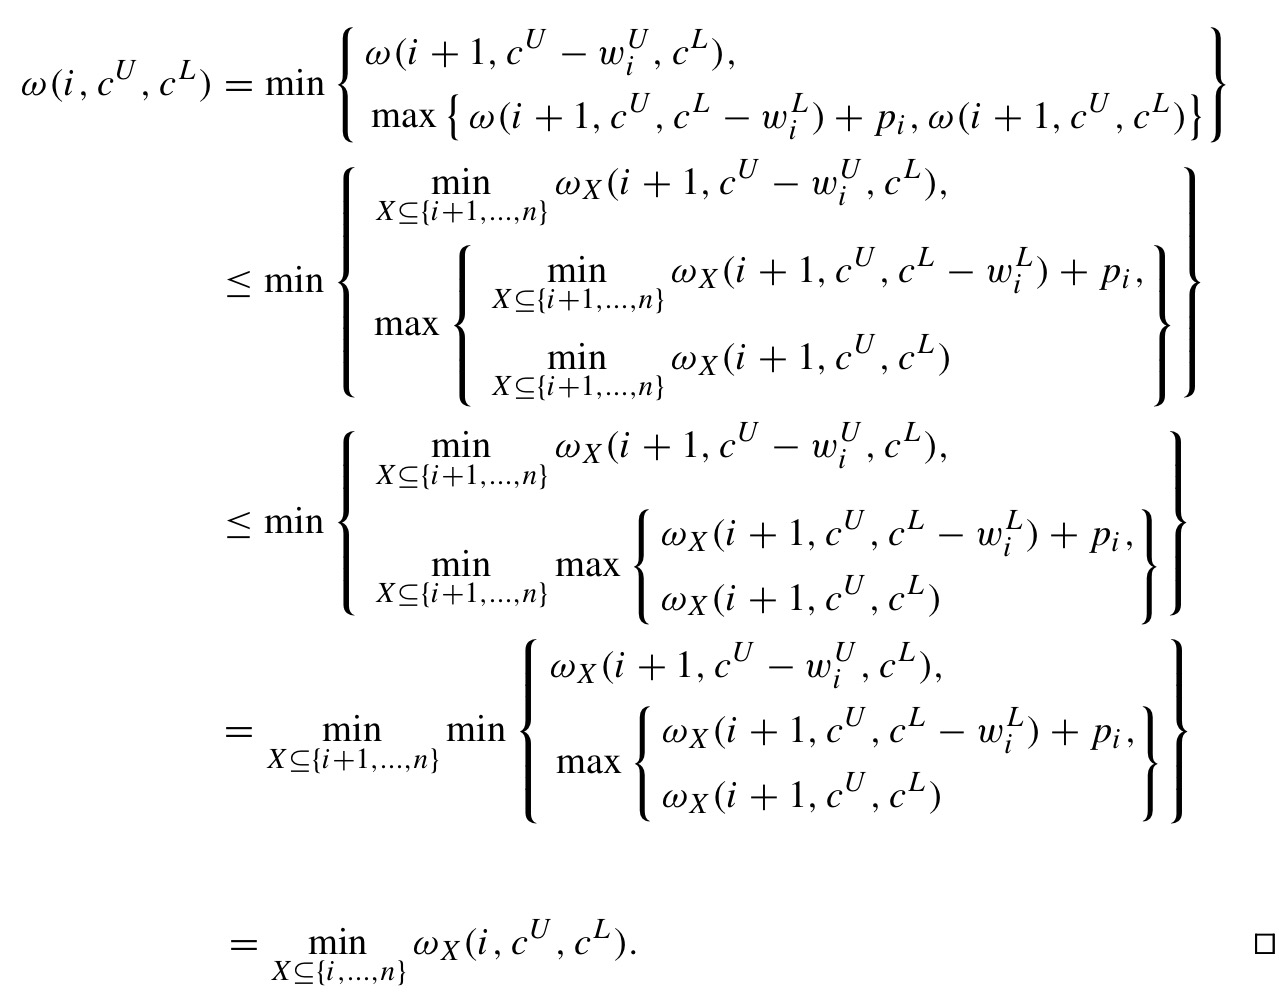
\includegraphics[width=0.8\linewidth]{ProofCase4.jpeg}
    \end{center}
\end{frame}

\begin{comment}
    


\begin{frame}{Case 4: $w_i^U \leq c^U$ and $w_i^L \leq c^L$}
\scalebox{0.65}{ % adjust scaling if needed
\begin{minipage}{\linewidth}
\begin{align*}
\omega(i, c^U, c^L) &= \min \left\{
\omega(i+1, c^U - w_i^U, c^L),\ 
\max \left\{
\omega(i+1, c^U, c^L - w_i^L) + p_i,\ 
\omega(i+1, c^U, c^L)
\right\}
\right\} \\
&\leq \min \left\{
\max \left\{
\min_{X \subseteq \{i+1, \ldots, n\}} \omega_X(i+1, c^U - w_i^U, c^L),\ 
\min_{X \subseteq \{i+1, \ldots, n\}} \left(
\omega_X(i+1, c^U, c^L - w_i^L) + p_i
\right),\right. \right. \\
&\hspace{6cm} \left. \left.
\min_{X \subseteq \{i+1, \ldots, n\}} \omega_X(i+1, c^U, c^L)
\right\}
\right\} \\
&\leq \min_{X \subseteq \{i+1, \ldots, n\}} 
\max \left\{
\omega_X(i+1, c^U, c^L - w_i^L) + p_i,\ 
\omega_X(i+1, c^U, c^L)
\right\} \\
&= \min_{X \subseteq \{i+1, \ldots, n\}} 
\omega_X(i, c^U, c^L) \\
&= \min_{X \subseteq \{i, \ldots, n\}} 
\omega_X(i, c^U, c^L). \\ \Box
\end{align*}
\end{minipage}
}
end{frame}

\end{comment}



\section{Tests and Analysis}





\begin{frame}[c]{Analysis}
\centering
\vspace{0.5cm}

\Large\textbf{Testing the Algorithm}



\end{frame}





\begin{frame}{Results Overview}
\scalebox{0.75}{
\begin{tabular}{l r r r r r r r r r}
\toprule
\textbf{Group} & \textbf{Num} & \multicolumn{4}{c}{\textbf{DCS}} & \multicolumn{4}{c}{\textbf{Comb}} \\
\cmidrule(lr){3-6} \cmidrule(lr){7-10}
& & Opt & Best & Avg & Max & Opt & Best & Avg & Max \\
\midrule
Uncorrelated           & 940 & 940 & 1  & 2.32    & 15.73   & 940 & 939 & 0.29   & 6.15 \\
Weak correlated        &  50 &  50 & 0  & 13.49   & 72.64   &  50 &  50 & 0.24   & 3.31 \\
Strong correlated      &  50 &  41 & 0  & 689.58  & 3600    &  50 &  50 & 0.32   & 4.18 \\
Inverse strong corr    &  50 &  38 & 0  & 919.91  & 3600    &  50 &  50 & 1.08   & 36.92 \\
Almost strong corr     &  50 &  40 & 0  & 815.4   & 3600    &  50 &  50 & 0.22   & 2.85 \\
Subset-sum             &  50 &  35 & 0  & 1087.18 & 3600    &  42 &  42 & 586.99 & 3600 \\
Even-odd subset-sum    &  50 &  36 & 0  & 1033.98 & 3600    &  42 &  42 & 581.63 & 3600 \\
Even-odd strong corr   &  50 &  41 & 0  & 747.12  & 3600    &  50 &  50 & 0.6    & 17.72 \\
Similar weight uncorr  &  50 &  50 & 0  & 22.89   & 79.85   &  50 &  50 & 0.04   & 0.09 \\
\bottomrule
\end{tabular}
}
\end{frame}



\begin{frame}{Performance in comparison with DCS}
    \begin{center}
        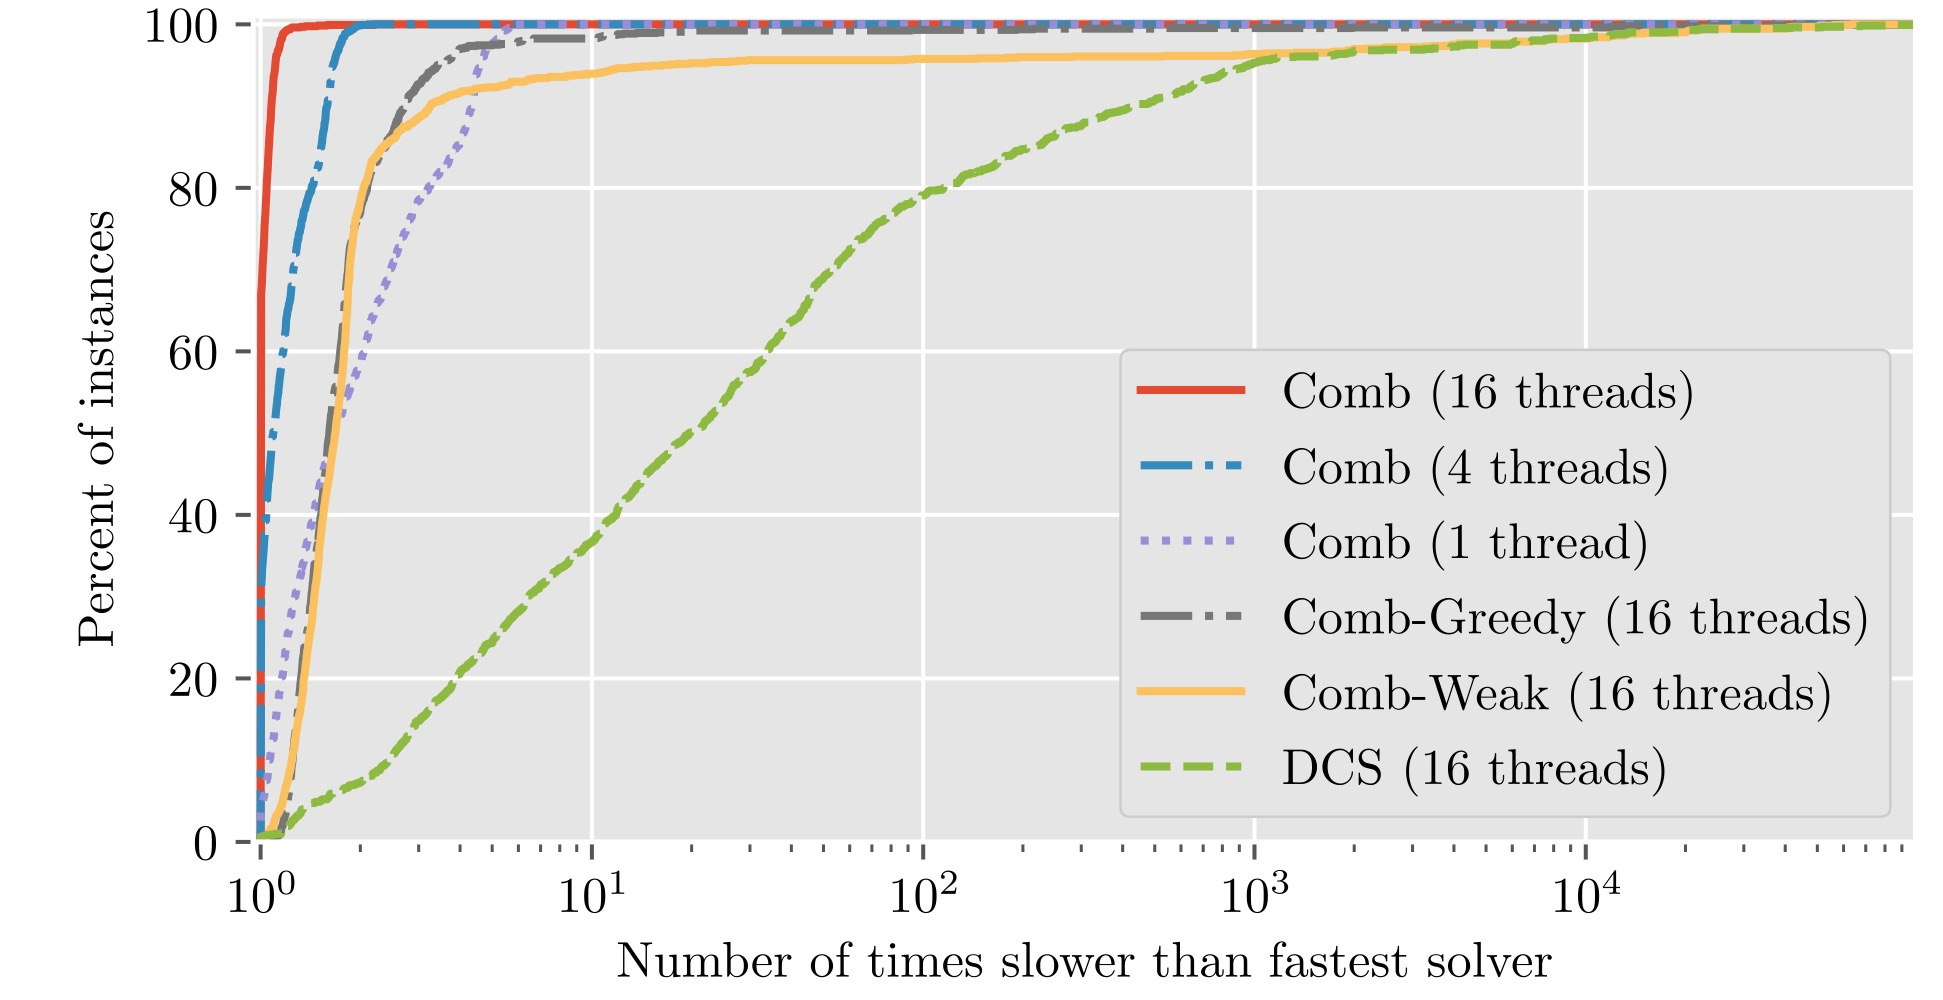
\includegraphics[width=0.9\linewidth]{Auswertung.jpeg}
        \small\textit{Performance Profile for all instances from the literature}
    \end{center}
    
\end{frame}






\begin{frame}{Table 4: Summary of Results for New Instances}
\scriptsize
\begin{tabularx}{\textwidth}{l r r r r r r r r r r}
\textbf{Group / $n$} & \textbf{Num} & \multicolumn{4}{c}{\textbf{DCS}} & \multicolumn{4}{c}{\textbf{Comb}} \\
& & Opt & Best & Avg & Max & Opt & Best & Avg & Max \\
\hline
$< 50$             & 660 & 583 & 2  & 116.61 & 900 & 660 & 658 & 0.02 & 0.24 \\
50                 & 250 & 203 & 0  & 178.63 & 900 & 247 & 247 & 17.55 & 900 \\
100                & 250 & 184 & 1  & 253.42 & 900 & 222 & 221 & 104.67 & 900 \\
1000               & 201 & 130 & 25 & 317.19 & 900 & 147 & 132 & 244.38 & 900 \\
10000              & 139 & 81  & 59 & 575.36 & 900 & 25  & 25  & 740.31 & 900 \\
\hline
Uncorrelated       & 269 & 256 & 16 & 73.05  & 900 & 243 & 242 & 87.81  & 900 \\
Lower subset-sum   & 273 & 174 & 2  & 354.32 & 900 & 236 & 235 & 124.88 & 900 \\
Upper subset-sum   & 267 & 261 & 30 & 54.78  & 900 & 236 & 231 & 105.24 & 900 \\
Both subset-sum    & 265 & 130 & 1  & 477.74 & 900 & 189 & 188 & 266.06 & 900 \\
Equal weights      & 266 & 265 & 38 & 32.92  & 900 & 237 & 227 & 98.77  & 900 \\
Large capacity     & 160 & 95  & 0  & 389.63 & 900 & 160 & 160 & 0.02   & 0.06 \\
\end{tabularx}
\end{frame}


\begin{frame}{DCS Results by $n$ and Group}
\scriptsize
\begin{tabularx}{\textwidth}{l r r r r}
\textbf{$n$ / Group} & \textbf{Num} & \textbf{Opt} & \textbf{Avg} & \textbf{Max} \\
\hline
\multicolumn{5}{l}{\textbf{DCS Results by $n$}} \\
1000         & 49  & 26 & 445.15 & 900 \\
10,000       & 111 & 66 & 473.96 & 900 \\
\hline
\multicolumn{5}{l}{\textbf{DCS Results by Group}} \\
Uncorrelated       & 31 & 26 & 360.55 & 900 \\
Lower subset-sum   & 27 & 0  & 900.00 & 900 \\
Upper subset-sum   & 33 & 33 & 134.08 & 265.25 \\
Both Subset-sum    & 35 & 0  & 900.00 & 900 \\
Equal weights      & 34 & 33 & 88.84  & 900 \\
\end{tabularx}
\end{frame}


\begin{frame}{Statisttics for Instances from the literature}
\scriptsize
\begin{tabularx}{\textwidth}{l R R R R R}
\textbf{Group} & \textbf{RootTime} & \textbf{OptTime} & \textbf{ProofTime} & \textbf{NumNodes} & \textbf{RootGap\%} \\
\hline
Uncorrelated           & 0.28 & 0.03 & 0.01 & 12,053.23      & 5.40 \\
Weak correlated        & 0.23 & 0.04 & 0.03 & 7,130.98       & 2.04 \\
Strong correlated      & 0.24 & 0.03 & 0.11 & 571,473.60     & 2.98 \\
Inverse strong corr    & 0.34 & 0.03 & 0.77 & 4,751,888.08   & 0.39 \\
Almost strong corr     & 0.21 & 0.03 & 0.03 & 735.76         & 2.99 \\
Subset-sum             & 0.07 & 0.04 & 13.05 & 104,067,718.79 & 0.02 \\
Even-odd subset-sum    & 0.07 & 0.04 & 6.67  & 61,246,957.64  & 0.02 \\
Even-odd strong corr   & 0.25 & 0.03 & 0.38  & 2,551,213.42   & 2.95 \\
Similar weight uncorr  & 0.04 & 0.04 & 0.04  & 0              & 0.00 \\
\end{tabularx}
\end{frame}


\begin{frame}{Statistics for newer Instances}
\scriptsize
\begin{tabularx}{\textwidth}{l R R R R R}
\textbf{Group} & \textbf{RootTime} & \textbf{OptTime} & \textbf{ProofTime} & \textbf{Nodes} & \textbf{RootGap\%} \\
\hline
Uncorrelated         & 0.82 & 0.26 & 0.17 & 73,616.37        & 9.86 \\
Lower subset-sum     & 0.94 & 0.79 & 3.21 & 11,293,085.12     & 1.27 \\
Upper subset-sum     & 0.84 & 0.00 & 0.00 & 187.94           & 5.72 \\
Both subset-sum      & 0.15 & 1.86 & 9.13 & 117,664,085.82    & 3.44 \\
Equal weights        & 0.73 & 0.02 & 0.02 & 14.59            & 1.64 \\
Large capacity       & 0.02 & 0.00 & 0.00 & 116.31           & 10.66 \\
\end{tabularx}
\end{frame}



\begin{frame}{Performance in comparison with DCS}
    \begin{center}
        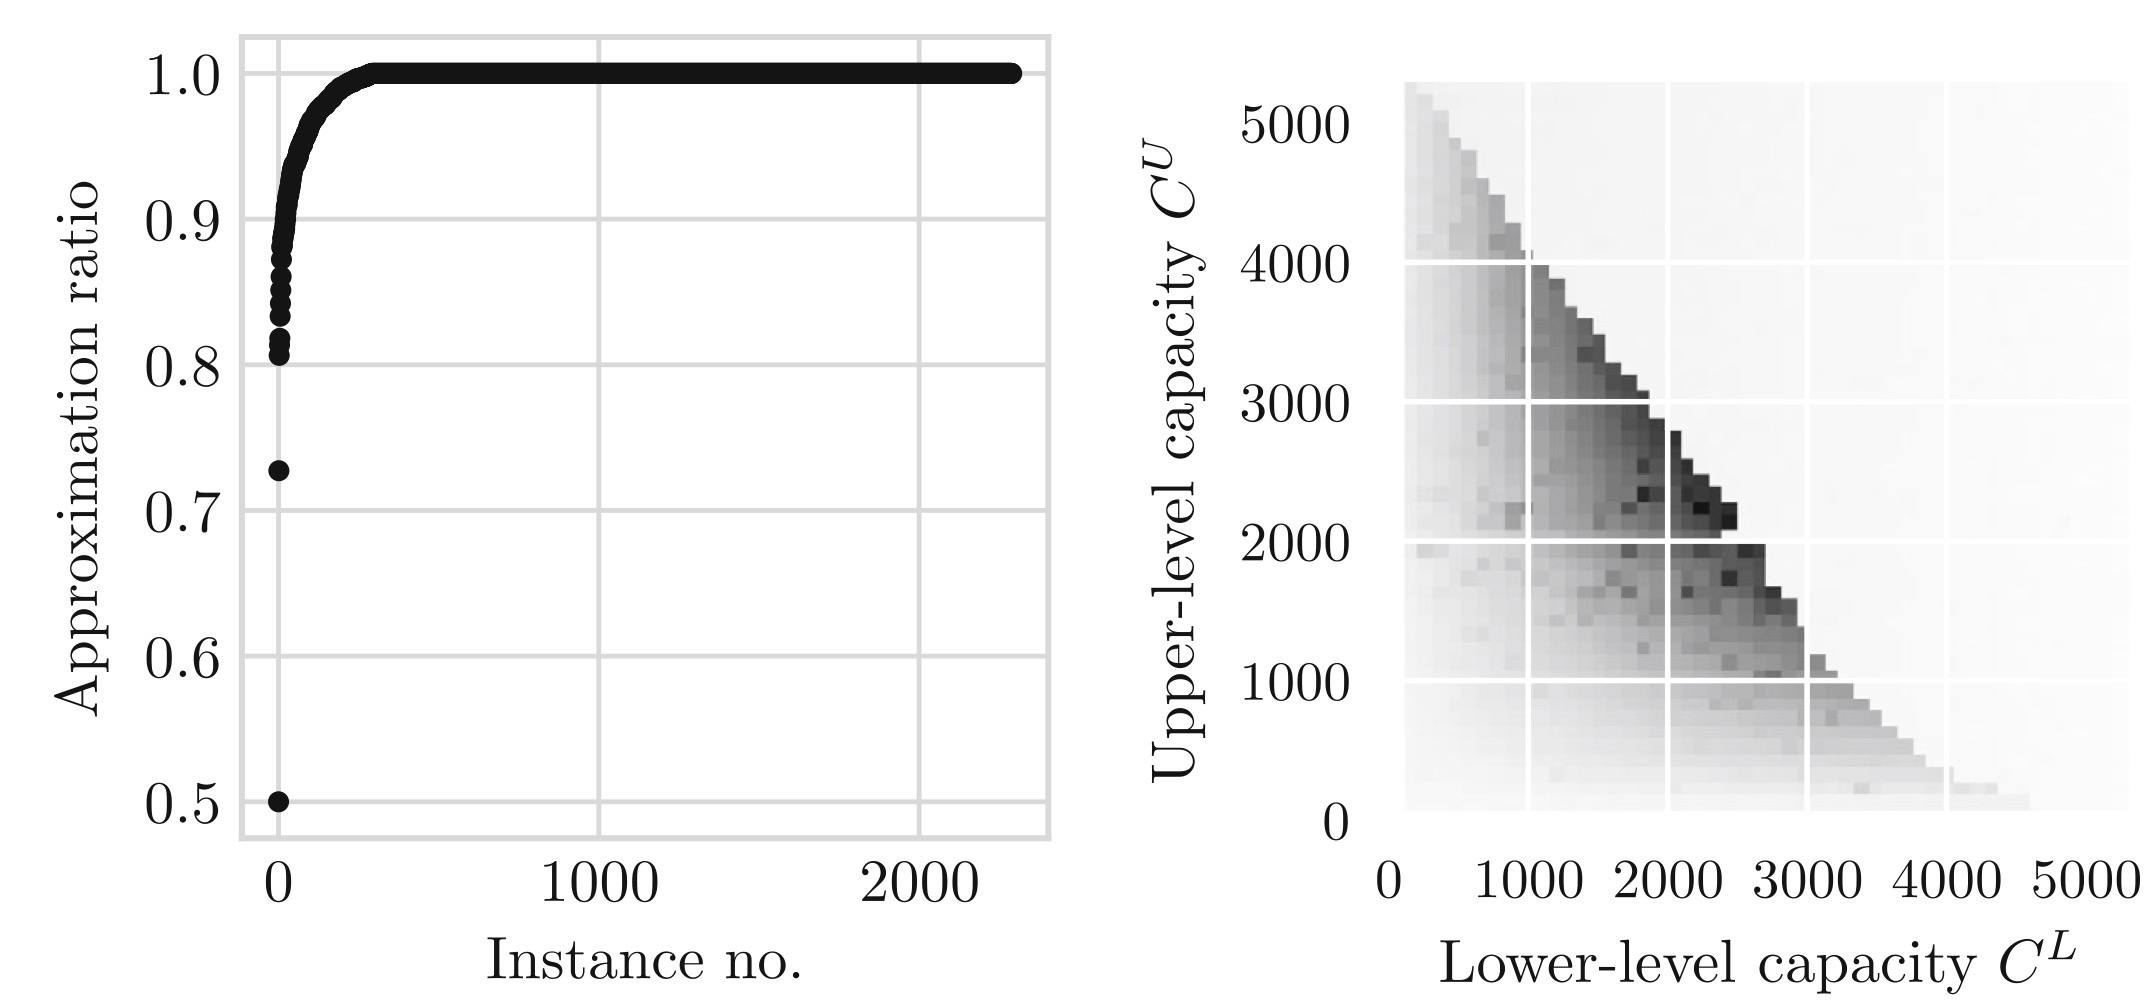
\includegraphics[width=0.9\linewidth]{ExtendedAnalysis.jpeg}
        %\small\textit{Performance Profile for all instances from the literature}
    \end{center}
\end{frame}


\begin{frame}{Quellenverzeichnis}
    \begin{itemize}
        \item Weninger, N., Fukasawa, R. A fast combinatorial algorithm for the bilevel knapsack problem with interdiction constraints. Math. Program. 210, 847–879 (2025). https://doi.org/10.1007/s10107-024-02133-9
   
        \item Matteo Fischetti, Michele Monaci, Markus Sinnl,
A dynamic reformulation heuristic for Generalized Interdiction Problems,
European Journal of Operational Research,
Volume 267, Issue 1,
2018,
Pages 40-51,
ISSN 0377-2217,
https://doi.org/10.1016/j.ejor.2017.11.043.

    \end{itemize}
\end{frame}
%[title={Literaturverzeichnis}, heading=bibintoc]




\title{End of the Presentation}
\subtitle{Thanks for listening}

\begin{frame}[plain]
\titlepage
\end{frame}

\end{document}
